% ============================================================
\chapter{Heat Equation}
\label{ch:heat}
% ============================================================

It was to understand the propagation of heat that Joseph Fourier developed the series that bear his name. His \emph{Th\'eorie analytique de la chaleur} (1822) is one of the founding texts of mathematical physics. The heat equation---the simplest parabolic PDE---describes an irreversible phenomenon: an initial temperature profile smooths over time, peaks flatten, gradients fade. Unlike the wave equation, information propagates at infinite speed, and unlike the transport equation, solutions become immediately smooth. These surprising, counter-intuitive properties make the heat equation the prototype of all diffusion equations.

\section{Physical motivation and formulation}

The heat equation describes thermal diffusion in a conducting medium.
If $u(x,t)$ represents the temperature, Fourier's law
($\vec{q} = -k\nabla u$) combined with energy conservation gives:

\begin{definition}[Heat equation]
The \textbf{heat equation} in dimension $n$ is:
\begin{equation}\label{eq:heat}
    u_t - \kappa\, \Delta u = f(x,t), \quad x \in \Omega \subset \R^n,\; t > 0,
\end{equation}
where $\kappa > 0$ is the thermal diffusivity. The case $f = 0$ is called
\textbf{homogeneous}.
\end{definition}

\begin{intuition}
The heat equation smooths out irregularities: even if the initial
temperature is discontinuous, the solution becomes instantaneously
$C^\infty$ for $t > 0$. This is the \textbf{smoothing effect} of
diffusion. However, information propagates at infinite speed (no wavefront).
\end{intuition}

\section{Fundamental solution}

\begin{definition}[Heat kernel]
The \textbf{heat kernel} (or fundamental solution) in dimension $n$ is:
\begin{equation}\label{eq:heat_kernel}
    \Phi(x,t) = \frac{1}{(4\pi\kappa t)^{n/2}}
    \exp\!\left(-\frac{\abs{x}^2}{4\kappa t}\right), \quad t > 0.
\end{equation}
\end{definition}

\begin{theorem}[Properties of the heat kernel]
The kernel $\Phi$ satisfies:
\begin{enumerate}
    \item $\Phi_t = \kappa\, \Delta \Phi$ for $t > 0$, $x \neq 0$.
    \item $\Phi(x,t) > 0$ for all $x \in \R^n$, $t > 0$.
    \item $\int_{\R^n} \Phi(x,t)\, dx = 1$ for all $t > 0$.
    \item $\Phi(\cdot, t) \to \delta_0$ in the sense of distributions as $t \to 0^+$.
\end{enumerate}
\end{theorem}

\begin{proof}
(1) Direct verification in dimension $n = 1$. We have
$\Phi(x,t) = (4\pi\kappa t)^{-1/2} e^{-x^2/(4\kappa t)}$. Computing:
\[
    \Phi_t = \Phi\left(-\frac{1}{2t} + \frac{x^2}{4\kappa t^2}\right),
    \quad
    \Phi_x = -\frac{x}{2\kappa t}\Phi, \quad
    \Phi_{xx} = \left(\frac{x^2}{4\kappa^2 t^2} - \frac{1}{2\kappa t}\right)\Phi.
\]
So $\Phi_t = \kappa\, \Phi_{xx}$.

(3) By the substitution $y = x/\sqrt{4\kappa t}$:
$\int_{\R^n} \Phi\, dx = \pi^{-n/2}\int_{\R^n} e^{-\abs{y}^2}\, dy = 1$.
\end{proof}

\begin{center}
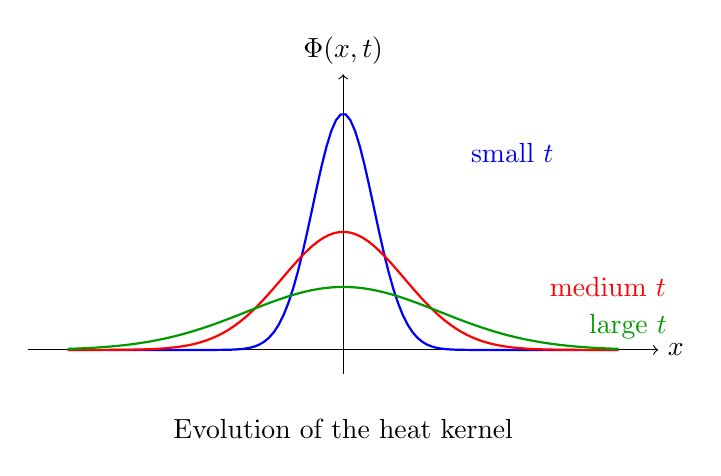
\begin{tikzpicture}[scale=1.0]
    \draw[->] (-4,0) -- (4,0) node[right] {$x$};
    \draw[->] (0,-0.3) -- (0,3.5) node[above] {$\Phi(x,t)$};
    % small t
    \draw[thick, blue, domain=-3:3, samples=100]
        plot (\x, {3*exp(-\x*\x/0.3)});
    \node[blue, right] at (1.5, 2.5) {small $t$};
    % medium t
    \draw[thick, red, domain=-3.5:3.5, samples=100]
        plot (\x, {1.5*exp(-\x*\x/1.2)});
    \node[red, right] at (2.5, 0.8) {medium $t$};
    % large t
    \draw[thick, green!60!black, domain=-3.5:3.5, samples=100]
        plot (\x, {0.8*exp(-\x*\x/3)});
    \node[green!60!black, right] at (3, 0.3) {large $t$};
    \node at (0, -1) {Evolution of the heat kernel};
\end{tikzpicture}
\end{center}

\section{Cauchy problem on $\R^n$}

\begin{theorem}[Solution by convolution]
If $u_0 \in L^\infty(\R^n) \cap C(\R^n)$, the solution of the Cauchy problem:
\[
    u_t = \kappa\, \Delta u, \quad u(x,0) = u_0(x),
\]
is given by convolution:
\begin{equation}\label{eq:cauchy_solution_heat}
    u(x,t) = (\Phi(\cdot, t) * u_0)(x)
    = \int_{\R^n} \Phi(x-y, t)\, u_0(y)\, dy.
\end{equation}
Moreover, $u \in C^\infty(\R^n \times (0,\infty))$.
\end{theorem}

\begin{proof}[Proof sketch]
One can differentiate under the integral sign because $\Phi$ is $C^\infty$
for $t > 0$ and decays exponentially. The initial condition follows from
property (4) of the kernel: $\Phi(\cdot, t) * u_0 \to u_0$ as $t \to 0^+$.
\end{proof}

\begin{keyformulas}[title=\textbf{Heat equation --- key formulas}]
\begin{itemize}
    \item Kernel ($n=1$): $\Phi(x,t) = \frac{1}{\sqrt{4\pi\kappa t}}\, e^{-x^2/(4\kappa t)}$.
    \item Cauchy solution: $u = \Phi * u_0$.
    \item With source: $u = \Phi * u_0 + \int_0^t \Phi(\cdot, t-s) * f(\cdot, s)\, ds$
          (Duhamel's formula).
\end{itemize}
\end{keyformulas}

\section{Maximum principle for the heat equation}

\begin{theorem}[Weak maximum principle]
Let $\Omega \subset \R^n$ be a bounded open set and
$\Omega_T = \Omega \times (0,T]$. If $u \in C^{2,1}(\Omega_T) \cap C(\overline{\Omega_T})$
satisfies $u_t - \kappa\Delta u \leq 0$ in $\Omega_T$, then:
\begin{equation}\label{eq:weak_max_heat}
    \max_{\overline{\Omega_T}} u = \max_{\Gamma_T} u,
\end{equation}
where $\Gamma_T = (\overline{\Omega} \times \{0\}) \cup (\partial\Omega \times [0,T])$
is the \textbf{parabolic boundary}.
\end{theorem}

\begin{proof}
Suppose by contradiction that the maximum is attained at an interior point
$(x_0, t_0) \in \Omega_T$ with $t_0 > 0$. Then $\nabla u(x_0, t_0) = 0$,
$D^2 u(x_0, t_0) \leq 0$ (negative semi-definite), so
$\Delta u(x_0, t_0) \leq 0$. Moreover, $u_t(x_0, t_0) \geq 0$ (since the
maximum is attained at $t_0$). Therefore
$u_t - \kappa\Delta u \geq 0$ at $(x_0, t_0)$, contradicting
$u_t - \kappa\Delta u \leq 0$ (unless equality). One concludes by
perturbation, considering $v = u - \varepsilon t$.
\end{proof}

\begin{center}
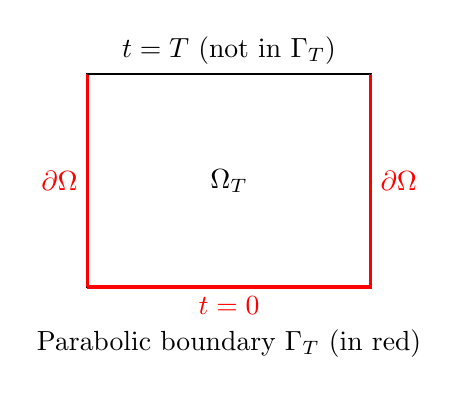
\begin{tikzpicture}[scale=0.9]
    \draw[thick] (0,0) rectangle (4,3);
    % Parabolic boundary in red
    \draw[very thick, red] (0,0) -- (4,0) -- (4,3);
    \draw[very thick, red] (0,0) -- (0,3);
    \draw[very thick, red] (0,0) -- (4,0);
    % Labels
    \node at (2, 1.5) {$\Omega_T$};
    \node[red, below] at (2, 0) {$t = 0$};
    \node[red, left] at (0, 1.5) {$\partial\Omega$};
    \node[red, right] at (4, 1.5) {$\partial\Omega$};
    \draw[dashed] (0,3) -- (4,3);
    \node[above] at (2,3) {$t = T$ (not in $\Gamma_T$)};
    \node at (2, -0.8) {Parabolic boundary $\Gamma_T$ (in red)};
\end{tikzpicture}
\end{center}

\begin{corollary}[Uniqueness]
The Cauchy--Dirichlet problem for the heat equation (on a bounded domain)
admits at most one classical solution.
\end{corollary}

\begin{proof}
If $u$ and $v$ are two solutions, $w = u - v$ satisfies $w_t = \kappa\Delta w$
with $w = 0$ on $\Gamma_T$. By the maximum principle, $w \leq 0$ in
$\overline{\Omega_T}$. Applying the same argument to $-w$, we get
$w \geq 0$, so $w = 0$.
\end{proof}

\section{Regularity and smoothing effect}

\begin{theorem}[Infinite regularity]
If $u$ solves $u_t = \kappa\Delta u$ in $\Omega_T$ with
$u_0 \in L^2(\Omega)$, then $u \in C^\infty(\Omega \times (0,T])$.
\end{theorem}

\begin{warning}[title=\textbf{Irreversibility}]
The heat equation is irreversible in time: one cannot, in general, go
backward in time. The problem $u_t = -\kappa\Delta u$ with final data is
ill-posed in the sense of Hadamard.
\end{warning}

\section{Asymptotic behaviour}

\begin{theorem}[Decay in time]
Let $u$ be the solution of $u_t = \kappa\Delta u$ on $\R^n$ with
$u_0 \in L^1(\R^n) \cap L^\infty(\R^n)$. Then:
\begin{enumerate}
    \item $\norm{u(\cdot,t)}_{L^\infty} \leq \frac{C}{t^{n/2}}\norm{u_0}_{L^1}$.
    \item $\norm{u(\cdot,t)}_{L^2}$ is decreasing in $t$.
    \item $\int_{\R^n} u(x,t)\, dx = \int_{\R^n} u_0(x)\, dx$ (mass conservation).
\end{enumerate}
\end{theorem}

\begin{proof}
(2) We compute:
\[
    \frac{d}{dt}\frac{1}{2}\int_{\R^n} u^2\, dx
    = \int_{\R^n} u\, u_t\, dx
    = \kappa\int_{\R^n} u\, \Delta u\, dx
    = -\kappa\int_{\R^n} \abs{\nabla u}^2\, dx \leq 0.
\]
(3) Integrating the equation and using the divergence theorem:
$\frac{d}{dt}\int u\, dx = \kappa\int \Delta u\, dx = 0$ (provided $u$
decays sufficiently at infinity).
\end{proof}

\section{Duhamel's formula}

\begin{theorem}[Duhamel's principle]
The solution of the inhomogeneous problem:
\[
    u_t - \kappa\Delta u = f(x,t), \quad u(x,0) = u_0(x),
\]
on $\R^n$ is:
\begin{equation}\label{eq:duhamel}
    u(x,t) = \int_{\R^n} \Phi(x-y,t)\, u_0(y)\, dy
    + \int_0^t \int_{\R^n} \Phi(x-y, t-s)\, f(y,s)\, dy\, ds.
\end{equation}
\end{theorem}

\begin{intuition}
Duhamel's principle is the PDE analogue of the variation of constants
method for ODEs. The source term $f$ is treated as a continuous
superposition of initial conditions applied at each instant $s$.
\end{intuition}

\section{Heat equation on a bounded interval}

\begin{example}
Solve completely:
\[
    \begin{cases}
        u_t = u_{xx}, & 0 < x < \pi,\; t > 0,\\
        u(0,t) = u(\pi,t) = 0,\\
        u(x,0) = x(\pi - x).
    \end{cases}
\]
By separation of variables (cf.\ Chapter~\ref{ch:fourier}), the eigenmodes
are $X_n = \sin(nx)$, $\lambda_n = n^2$, and:
\[
    u(x,t) = \sum_{n=1}^{\infty} b_n \sin(nx)\, e^{-n^2 t}.
\]
The Fourier sine coefficients of $f(x) = x(\pi-x)$ are:
\[
    b_n = \frac{2}{\pi}\int_0^\pi x(\pi-x)\sin(nx)\, dx
    = \begin{cases} \frac{8}{n^3\pi} & \text{if $n$ odd,}\\ 0 & \text{if $n$ even.}\end{cases}
\]
Therefore:
\[
    u(x,t) = \frac{8}{\pi}\sum_{k=0}^{\infty}
    \frac{\sin((2k+1)x)}{(2k+1)^3}\, e^{-(2k+1)^2 t}.
\]
For large $t$, $u(x,t) \approx \frac{8}{\pi}\sin(x)\, e^{-t}$:
only the first mode survives.
\end{example}

\section{Inhomogeneous boundary conditions}

To handle $u(0,t) = g_0(t)$, $u(L,t) = g_1(t)$, we set
$v(x,t) = u(x,t) - w(x,t)$ where $w$ is a \textbf{lifting} of the
boundary conditions:
\[
    w(x,t) = g_0(t) + \frac{x}{L}\bigl(g_1(t) - g_0(t)\bigr).
\]
Then $v$ satisfies the heat equation with homogeneous conditions and a
modified source term.

\section{Exercises}

\begin{exercise}
Verify that $\Phi(x,t) = \frac{1}{\sqrt{4\pi\kappa t}}\, e^{-x^2/(4\kappa t)}$
satisfies $\Phi_t = \kappa\, \Phi_{xx}$ for $t > 0$.
\end{exercise}

\begin{exercise}
Solve $u_t = u_{xx}$ on $\R$ with $u(x,0) = e^{-\abs{x}}$.
\end{exercise}

\begin{exercise}
Show that the energy $E(t) = \frac{1}{2}\int_0^L u^2(x,t)\, dx$ is
decreasing for the heat equation with homogeneous Dirichlet conditions.
What is the rate of decay?
\end{exercise}

\begin{exercise}
Solve $u_t = u_{xx} + \sin(x)$ on $(0,\pi)$ with $u(0,t) = u(\pi,t) = 0$
and $u(x,0) = 0$. \emph{Hint:} look for a stationary solution, then use
Duhamel.
\end{exercise}

\begin{exercise}
Let $u$ solve $u_t = u_{xx}$ on $(0,1)$ with $u(0,t) = 0$, $u(1,t) = 1$,
$u(x,0) = x$. Find the stationary solution and show that $u$ converges
to it.
\end{exercise}

\begin{exercise}[Self-similarity]
Look for a solution of $u_t = u_{xx}$ of the form
$u(x,t) = t^{-\alpha} f(\xi)$ with $\xi = x/\sqrt{t}$.
Determine $\alpha$ and the ODE satisfied by $f$.
\end{exercise}

\begin{exercise}
Show that the maximum temperature decreases over time for the heat
equation on a bounded domain with homogeneous Dirichlet conditions.
\emph{Hint:} use the maximum principle.
\end{exercise}
